\begin{frame}{Modèle de langage}
Un modèle de langage a pour but d’estimer la probabilité a priori de toutes les séquences de mots qu’il est
possible de construire à partir du lexique. Pour ce faire, il peut s’appuyer sur différentes
sources d’informations, comme par exemple des règles syntaxiques ou sémantiques, ou
encore des statistiques issues de gros volumes de données. On se concentre ici
sur les modèles de langages statistiques.
\end{frame}


\begin{frame}{Modèle des N-Grammes}
Principe : L’idée à la base des modèles de langage n-gramme est que la probabilité d’apparition
d’un mot peut être estimée à partir des n-1 mots le précédant. On peut ainsi faire
une approximation sur le contexte utilisé pour le calcul des probabilités conditionnelles
de la formule suivante:

\begin{figure}
\centering
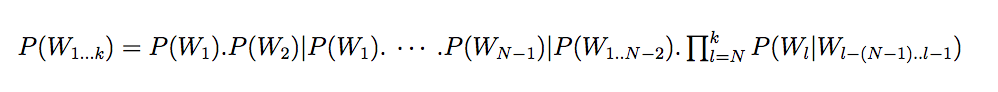
\includegraphics[width=10cm]{images/modele_langage.png}
\end{figure}

\end{frame}

\begin{frame}{Création de Modèle de langage en utilisant CMUCLMTK}
La création d'un Modèle de langage statistique peut se résumer en trois étapes:
\begin{itemize}
\item Collecter des textes
\item Transformer les textes en corpus
\item Transformer le corpus en une distribution de probabilités
\end{itemize}
\end{frame}

